\documentclass{book}

\usepackage{amsmath, mathrsfs, amssymb, bbm, amsthm, enumitem, times, mathtools, tikz, mathptmx, xcolor, wrapfig}
\usepackage[framemethod=tikz]{mdframed}
\usepackage[margin=4cm]{geometry}

\usetikzlibrary{cd, decorations.markings, arrows}

\newcommand{\scrA}{\mathscr{A}}
\newcommand{\scrB}{\mathscr{B}}
\newcommand{\scrC}{\mathscr{C}}
\newcommand{\scrD}{\mathscr{D}}
\newcommand{\scrE}{\mathscr{E}}
\newcommand{\scrF}{\mathscr{F}}
\newcommand{\scrL}{\mathscr{L}} 
\newcommand{\scrN}{\mathscr{N}}
\newcommand{\bbE}{\mathbb{E}}
\newcommand{\bbN}{\mathbb{N}}
\newcommand{\bbP}{\mathbb{P}}
\newcommand{\bbR}{\mathbb{R}}
\newcommand{\bbRP}{\mathbb{RP}}
\newcommand{\bbT}{\mathbb{T}}
\newcommand{\bbZ}{\mathbb{Z}}
\newcommand{\bbZmod}[1]{\bbZ/{#1}\bbZ}
\newcommand{\bbone}{\mathbbm{1}}
\renewcommand{\d}{\mathrm{d}}
\newcommand{\e}{\mathrm{e}}
\renewcommand{\i}{\mathrm{i}}
\renewcommand{\epsilon}{\varepsilon}
\renewcommand{\phi}{\varphi}

\newcommand{\abs}[1]{\left\vert {#1} \right\vert}
\newcommand{\norm}[1]{\left\Vert {#1} \right\Vert}
\newcommand{\set}[1]{\left\{ {#1} \right\}}
\newcommand{\parens}[1]{\left( {#1} \right)}
 
\newcommand{\distributionEqual}{\overset{\scrD}{=}}
\newcommand{\iidEqual}{\overset{\mathrm{i.i.d.}}{=}}
\newcommand{\weak}{\rightharpoonup}

\newcommand{\consum}{\mathop{\vcenter{\hbox{\LARGE\#}}}\limits}
%\newcommand{\consum}{\mathop{\mathchoice
%  {\vcenter{\hbox{\LARGE$\#$}}}
%  {\vcenter{\hbox{\large$\#$}}}
%  {\vcenter{\hbox{\footnotesize$\#$}}}
%  {\vcenter{\hbox{\scriptsize$\#$}}}
%}\displaylimits}

\DeclareMathOperator{\dom}{dom}
\DeclareMathOperator{\im}{im}
\DeclareMathOperator{\id}{id}
\DeclareMathOperator{\pr}{pr}
\DeclareMathOperator{\Ob}{Ob}
\DeclareMathOperator{\Hom}{Hom}
\DeclareMathOperator{\Ext}{Ext}
\DeclareMathOperator{\rank}{rank}

\DeclareRobustCommand{\coprod}{\mathop{\text{\fakecoprod}}}
\newcommand{\fakecoprod}{%
  \sbox0{$\prod$}%
  \smash{\raisebox{\dimexpr.9625\depth-\dp0}{\scalebox{1}[-1]{$\prod$}}}%
  \vphantom{$\prod$}%
}

\newtheorem{theorem}{Theorem}[section]
\newtheorem{proposition}[theorem]{Proposition}
\newtheorem{lemma}[theorem]{Lemma}
\newtheorem{corollary}[theorem]{Corollary}

\theoremstyle{definition}
\newtheorem{example}[theorem]{Example}

\theoremstyle{remark}
\newtheorem{remark}[theorem]{Remark}

\surroundwithmdframed[outerlinewidth=0.4pt,middlelinewidth=1pt,innerlinewidth=0.4pt,middlelinecolor=white,bottomline=false,topline=false,rightline=false,innertopmargin=-9pt,innerbottommargin=-1pt]{theorem}
\surroundwithmdframed[outerlinewidth=0.4pt,bottomline=false,topline=false,rightline=false,innertopmargin=-9pt,innerbottommargin=-1pt]{lemma}
\surroundwithmdframed[outerlinewidth=0.4pt,bottomline=false,topline=false,rightline=false,innertopmargin=-9pt,innerbottommargin=-1pt]{proposition}
\surroundwithmdframed[outerlinewidth=0.4pt,bottomline=false,topline=false,rightline=false,innertopmargin=-9pt,innerbottommargin=-1pt]{corollary}
%\surroundwithmdframed[tikzsetting={draw=black,line width=1pt,dashed},bottomline=false,topline=false,rightline=false,innertopmargin=-5pt,outerlinecolor=white,middlelinecolor=white]{example}

\numberwithin{equation}{section}

\title{Cohomology} 
\author{Billy Sumners}

\begin{document}
\maketitle 

\chapter{Introduction}
\section{Motivation}

\section{Review of Homological Algebra}
A \textit{chain complex} $C_*$ is a sequence $(C_k, \partial_k)_{k \in \bbZ}$ of abelian groups $C_k$, called \textit{chain groups} and homomorphisms $\partial_k \colon C_k \to C_{k-1}$, called \textit{boundary maps} such that $\partial_{k-1} \circ \partial_k = 0$ for all $k \in \bbZ$. The integer $k$ is called the \textit{degree} of the chain group $C_k$ in $C_*$. When clear from context, we will avoid writing the $k$ in $\partial_k$. For example, with this convention, our condition on being a boundary map becomes $\partial^2 = 0$. A chain complex is often denoted by
\begin{equation}
    \begin{aligned}
        C_*: 
        & 
        \begin{tikzcd}
            \cdots \arrow[r] & C_{k+1} \arrow[r,"\partial_{k+1}"] & C_k \arrow[r,"\partial_k"] & C_{k-1} \arrow[r] & \cdots.
        \end{tikzcd} 
        & 
        \hphantom{ }
    \end{aligned} 
\end{equation}

A chain complex $C_*$ is \textit{finite-dimensional} if $C_k \neq 0$ for at most finitely many $k$. It is \textit{locally finite} if $C_k$ is finitely generated for all $k$, and it is \textit{finite} if it is both finite-dimensional and locally finite.

Elements of $C_k$ are called $k$\textit{-chains} or \textit{chains of degree} $k$. Elements of $Z_k(C_*) := \ker{\partial_k}$ are called $k$\textit{-cycles} or \textit{cycles of degree} $k$, and elements of $B_k(C_*) := \im{\partial_{k+1}}$ are called $k$\textit{-boundaries} or \textit{boundaries of degree} $k$. The \textit{homology groups} of $C_*$ are the quotient groups $H_k(C_*) := Z_k(C_*) / B_k(C_*)$.

Given chain complexes $C_*$ and $D_*$, a \textit{chain map} $f \colon C_* \to D_*$ is a sequence of homomorphisms $f_k \colon C_k \to D_k$ such that $f_{k-1} \circ \partial_k^{C} = \partial_k^{D} \circ f_k$. Thus there is a commutative diagram 
\begin{equation}
    \begin{tikzcd}
        \cdots \arrow[r] & C_{k+1} \arrow[r,"\partial_{k+1}^C"] \arrow[d,"f_{k+1}"] & C_k \arrow[r,"\partial_k^C"] \arrow[d,"f_k"] & C_{k-1} \arrow[d,"f_{k-1}"] \arrow[r] & \cdots \\
        \cdots \arrow[r] & D_{k+1} \arrow[r,"\partial_{k+1}^D"]                     & D_k \arrow[r,"\partial_k^D"]                 & D_{k-1} \arrow[r]                     & \cdots              
    \end{tikzcd}
\end{equation}
A chain map is a \textit{chain isomorphism} if each homomorphism $f_k$ is an isomorphism.

A chain complex $C_*$ is \textit{exact} if $H_k(C_*) = 0$ for all $k$. That is, $Z_k(C_*) = B_k(C_*)$ for all $k$. In this context, we usually say $C_*$ is an \textit{exact sequence} rather than an exact chain complex. An exact sequence $C_*$ is \textit{short} (abbreviated s.e.s.) if it is of the form 
\begin{equation}
    \begin{tikzcd}
        0 \arrow[r] & A \arrow[r] & B \arrow[r] & C \arrow[r] & 0
    \end{tikzcd}
\end{equation}

\begin{example}
    We will calculate the homology of the following sequences, and in particular, see which are exact.
    \begin{enumerate}[label=(\arabic*)]
        \item
        \begin{tikzcd}
                0 \arrow[r] & \bbZ \arrow[r] & 0
        \end{tikzcd}
        \item For $n \in \bbZ$,
        \begin{tikzcd}
            0 \arrow[r] & \bbZ \arrow[r,"\cdot n"] & \bbZ \arrow[r] & 0
        \end{tikzcd}
        \item 
        \begin{tikzcd}
            0 \arrow[r] & \bbZ \arrow[r,"\cdot 2"] & \bbZ \arrow[r] & \bbZ/2\bbZ \arrow[r] & 0
        \end{tikzcd}
    \end{enumerate}
\end{example}

Let $C_*$ and $D_*$ be chain complexes. The \textit{direct sum} of $C_*$ and $C_*$ is the chain complex $C_* \oplus D_*$ with chain groups $C_k \oplus D_k$ and boundary maps $\partial := \partial^C \oplus \partial^D$, defined more precisely by $\partial(c,d) := (\partial^C c, \partial^D d)$.

\begin{example}
    Suppose $C_*$ and $D_*$ are the chain complexes
    \begin{equation} \begin{aligned}
        C_*:  &
        \begin{tikzcd}
            \overset{4}{0} \arrow[r] & \overset{3}{\bbZ} \arrow[r,"\id"] & \overset{2}{\bbZ} \arrow[r] & \overset{1}{0}
        \end{tikzcd}
        & \hphantom{ } \\
        D_*:  &
        \begin{tikzcd}
            \overset{3}{0} \arrow[r] & \overset{2}{\bbZ} \arrow[r,"\id"] & \overset{1}{\bbZ} \arrow[r] & \overset{1}{0}
        \end{tikzcd}
        & \hphantom{ }
    \end{aligned} \end{equation}
    where we have denoted the degree of the corresponding chain maps by the numbers overhead. The chain complex $C_* \oplus D_*$ is then
    \begin{equation}
        \begin{tikzcd}
            \overset{4}{0} \arrow[r] & \overset{3}{\bbZ} \arrow[r,"{(\id,0)}"] & \overset{2}{\bbZ^2} \arrow[r,"\pr_2"] & \overset{1}{\bbZ} \arrow[r] & \overset{0}{0}
        \end{tikzcd}
    \end{equation}
    The map $\pr_i \colon \bbZ^n \to \bbZ$ denotes projection onto the $i$th component. 

    This example stresses the importance of knowing the degree of each chain group. If we had put our chain groups in different positions, we would obtain entirely different chain complexes!
\end{example}

\begin{proposition}
    \begin{enumerate}[label={\rm(\arabic*)}]
        \item Let $C_*$ and $D_*$ be chain complexes. Then $H_k(C_* \oplus D_*) \cong H_k(C_*) \oplus H_k(D_*)$ for all $k \in \bbZ$.
        \item Suppose $C_*$ is finite and free, in the sense that all its chain groups are free abelian groups. Then $C_*$ is a finite sum of copies of sequences of the form 
        \begin{equation}
            \begin{tikzcd}
                0 \arrow[r] & \overset{k}{\bbZ} \arrow[r,"\cdot m_k"] & \overset{k-1}{\bbZ} \arrow[r] & \cdots \arrow[r] & \overset{l}{\bbZ} \arrow[r,"\cdot m_l"] & \overset{l-1}{\bbZ} \arrow[r] & 0
            \end{tikzcd}
        \end{equation}
        for $l \leq k$ and $m_l, m_{l+1}, \dots, m_k \neq 0$.
    \end{enumerate}
\end{proposition}

A short exact sequence 
\begin{tikzcd}[cramped,sep=small]
    0 \arrow[r] & A \arrow[r,"i"] & B \arrow[r,"j"] & C \arrow[r] & 0
\end{tikzcd}
is said to \textit{split} if there exists an isomorphism $B \cong A \oplus C$ such that the following diagram commutes.
\begin{equation}
    \begin{tikzcd}
                    &                                                           & B \arrow[dd,"\cong"] \arrow[rd,"j" description] &             &   \\
        0 \arrow[r] & A \arrow[ru,"i" description] \arrow[rd,"i_A" description] &                                                 & C \arrow[r] & 0 \\
                    &                                                           & A \oplus C \arrow[ru,"\pr_B" description]       &             & 
    \end{tikzcd}
\end{equation}
Here, $i_A$ denotes the natural inclusion of $A$ in $A \oplus C$. Recall the following lemma 
\begin{lemma}[Splitting]
    Let $C_*:$
    \begin{tikzcd}[cramped,sep=small]
        0 \arrow[r] & A \arrow[r,"i"] & B \arrow[r,"j"] & C \arrow[r] & 0
    \end{tikzcd}
    be a short exact sequence. The following are equivalent:
    \begin{enumerate}[label={\rm(\roman*)}]
        \item The sequence $C_*$ splits.
        \item There exists a homomorphism $s \colon C \to B$ such that $j \circ s = \id_C$.
        \item There exists a homomorphism $r \colon B \to A$ such that $r \circ i = \id_A$.
    \end{enumerate}
    Thus if $C$ is a free group, then $C_*$ splits.
\end{lemma}

\begin{example}
    We show the splitting properties of the following sequences.
    \begin{enumerate}[label=(\arabic*)]
        \item The sequence 
        \begin{tikzcd}[cramped,sep=small]
            0 \arrow[r] & \bbZ/2\bbZ \arrow[r,"\cdot 2"] & \bbZ/4\bbZ \arrow[r] & \bbZ/2\bbZ \arrow[r] & 0
        \end{tikzcd}
        doesn't split.
        \item The sequence
        \begin{tikzcd}[cramped,sep=small]
            0 \arrow[r] & \bbZ/3\bbZ \arrow[r,"\cdot 2"] & \bbZ/6\bbZ \arrow[r] & \bbZ/2\bbZ \arrow[r] & 0
        \end{tikzcd}
        splits uniquely.
        \item The sequence
        \begin{tikzcd}[cramped,sep=small]
            0 \arrow[r] & \bbZ/2\bbZ \arrow[r,"i_1"] & \bbZ/2\bbZ \oplus \bbZ/2\bbZ \arrow[r,"\pr_2"] & \bbZ/2\bbZ \arrow[r] & 0
        \end{tikzcd}
        splits in two ways.
    \end{enumerate}
\end{example}

        
\chapter{Cohomology and the Universal Coefficient Theorem}
\section{The Hom Functor}
Before we can go any further, we need to take a short digression to introduce functors.

A \textit{category} $\scrC$ consists of the following data:
\begin{enumerate}[label=(\arabic*)]
    \item A collection $\Ob(\scrC)$ of \textit{objects},
    \item for any $A,B \in \Ob(\scrC)$, a collection $\Hom(A,B)$ of \textit{morphisms} (also called \textit{arrows}),
    \item for any $A \in \Ob(\scrC)$, a special \textit{identity morphism} $\id_A \in \Hom(A,A)$,
    \item for any $A,B,C \in \Ob(\scrC)$, a composition rule $\circ \colon \Hom(B,C) \times \Hom(A,B) \to \Hom(A,C)$,
\end{enumerate}
such that 
\begin{enumerate}[label=(\alph*)]
    \item for all $A,B \in \Ob(\scrC)$ and $f \in \Hom(A,B)$, we have $f \circ \id_A = f$ and $\id_B \circ f = f$.
    \item for all $A,B,C,D \in \Ob(\scrC)$ and $f \in \Hom(A,B)$, $g \in \Hom(B,C)$, and $h \in \Hom(C,D)$, we have $h \circ (g \circ f) = (h \circ g) \circ f$.
\end{enumerate}
It is common to write $A \in \scrC$ in place of $A \in \Ob(\scrC)$, and $f \colon A \to B$ in place of $f \in \Hom(A,B)$.

\begin{example}
    We give some examples of categories.
    \begin{enumerate}[label=(\arabic*)]
        \item The category $\mathrm{Set}$ of sets and functions between them.
        \item The category $\mathrm{Gp}$ of groups and homomorphisms between them.
        \item The category $\mathrm{Ab}$ of abelian groups and homomorphisms between them. This category is in face a \textit{subcategory} of $\mathrm{Gp}$, in the sense that it is obtained from $\mathrm{Gp}$ by deleting some objects and morphisms.
        \item The category $\mathrm{Vect}_k$ of vector spaces over a field $k$ and linear maps between them.
        \item The category $\mathrm{Top}$ of topological spaces and continuous maps between them.
        \item The category $\mathrm{Top_*}$ of pointed topological spaces and pointed maps between them.
    \end{enumerate}
\end{example}

Let $\scrC$ and $\scrD$ be categories. A \textit{covariant functor} $\scrF \colon \scrC \to \scrD$ consists of 
\begin{enumerate}[label=(\arabic*)]
    \item a map $\Ob(\scrC) \to \Ob(\scrD)$,
    \item for any $A,B \in \scrC$, a map $\Hom(A,B) \to \Hom(\scrF(A),\scrF(B))$
\end{enumerate}
such that 
\begin{enumerate}[label=(\alph*)]
    \item for all $A \in \scrC$, we have $\scrF(\id_A) = \id_{\scrF(A)}$,
    \item for all $A,B,C \in \scrC$ and $f \in \Hom(A,B)$, $g \in \Hom(B,C)$, we have $\scrF(g \circ f) = \scrF(g) \circ \scrF(f)$.
\end{enumerate}
A \textit{contravariant functor} is the same sort of thing, except the functor reverses the arrows. That is, $\scrF$ maps $\Hom(A,B)$ to $\Hom(\scrF(B),\scrF(A))$, and (b) is replaced by $\scrF(g \circ f) = \scrF(f) \circ \scrF(g)$.
\begin{example}
    The fundamental group $\pi_1 \colon \mathrm{Top}_* \to \mathrm{Gp}$ is a covariant functor, and dualization $\mathrm{Vect}_k \to \mathrm{Vect}_k$ given by $V \mapsto V^* = \Hom_k(V,k)$ is a contravariant functor.
\end{example}

For a fixed abelian group $G$, two of the most important functors we will consider are the covariant functor $\Hom(G,\cdot) \colon \mathrm{Ab} \to \mathrm{Ab}$, and the contravariant functor $\Hom(\cdot,G) \colon \mathrm{Ab} \to \mathrm{Ab}$. In particular, for $\phi \in \Hom(A,B)$, we can define the homomorphism $\phi_* \colon \Hom(G,A) \to \Hom(G,B)$ by $(\phi_* f)(g) = \phi(f(g))$, and the homomorphism $\phi^* \colon \Hom(B,G) \to \Hom(A,G)$ by $(\phi^*f)(a) = f(\phi(a))$.
\begin{lemma}
    \begin{enumerate}[label=\rm{(\arabic*)}]
        \item For abelian groups $A,B,G$, we have 
        \begin{equation}
            \Hom(A \oplus B, G) \cong \Hom(A,G) \oplus \Hom(B,G),
        \end{equation}
        and 
        \begin{equation}
            \Hom(G,A \oplus B) \cong \Hom(G,A) \oplus \Hom(G,B).
        \end{equation}
        \item For any abelian group $A$, we have $\Hom(\bbZ,A) \cong A$.
        \item For any finitely generated abelian group $A$, $\Hom(A,\bbZ)$ is isomorphic to the free part of $A$.
    \end{enumerate}
\end{lemma}

A \textit{cochain complex} is a sequence $(C^k,\delta^k)_{k \in \bbZ}$ of abelian groups $C^k$, called \textit{cochain groups}, and homomorphisms $\delta^k \colon C^{k-1} \to C^k$, called \textit{coboundary maps}, such that $\delta^{k+1} \circ \delta^k = 0$. Elements of $C^k$ are called \textit{cochains}, elements of $Z^k(C^*) := \ker{\delta^{k+1}}$ are called \textit{cocycles}, and elements of $B^k(C^*) := \im{\delta^k}$ are called \textit{coboundaries}. The \textit{cohomology} of $C^*$ is defined by $H^k(C^*) := Z^k(C^*)/B^k(C^*)$.

Fix an abelian group $G$. Given a chain complex
\begin{equation}
    \begin{aligned}
        C_*: 
        & 
        \begin{tikzcd}
            \cdots \arrow[r] & C_{k+1} \arrow[r,"\partial_{k+1}"] & C_k \arrow[r,"\partial_k"] & C_{k-1} \arrow[r] & \cdots,
        \end{tikzcd} 
        & 
        \hphantom{ }
    \end{aligned} 
\end{equation}
we can construct from it a cochain complex by applying the contravariant functor $\Hom(\cdot,G)$. That is, 
\begin{equation} \label{eq:dualOfAChainComplex}
    \begin{aligned}
        C^* = \Hom(C_*,G): 
        & 
        \begin{tikzcd}
            \cdots & C^{k+1} \arrow[l] & C^k \arrow[l,"\delta^{k+1}" above] & C^{k-1} \arrow[l,"\delta^k" above] & \cdots \arrow[l],
        \end{tikzcd} 
        & 
        \hphantom{ }
    \end{aligned} 
\end{equation}
where $C^k = \Hom(C_k,G)$, and $\delta^k(\phi) := \phi\circ\partial_k$. The \textit{cohomology of} $C_*$ \textit{with coefficients in} $G$ is defined to be the cohomology of $C^*$, and is denoted $H^k(C_*,G)$. As with homology, cohomology is functorial. Indeed, suppose $\alpha \colon C_* \to D_*$ is a chain map. That is, we have a commutative diagram 
\begin{equation} \begin{tikzcd}
    \cdots \arrow[r] & C_{k+1} \arrow[r,"\partial"] \arrow[d,"\alpha_{k+1}"] & C_{k} \arrow[r,"\partial"] \arrow[d,"\alpha_{k}"] & C_{k-1} \arrow[r] \arrow[d,"\alpha_{k-1}"] & \cdots \\
    \cdots \arrow[r] & D_{k+1} \arrow[r,"\partial"]                          & D_{k} \arrow[r,"\partial"]                        & D_{k-1} \arrow[r]                          & \cdots
\end{tikzcd} \end{equation}
Dualizing this sequence via the contravariant functor $\Hom(\cdot,G)$, we obtain 
\begin{equation} \begin{tikzcd}
    \cdots & C^{k+1} \arrow[l]                          & C^{k} \arrow[l,"\delta"]                        & C_{k-1} \arrow[l,"\delta"]                          & \cdots \arrow[l] \\
    \cdots & D^{k+1} \arrow[l] \arrow[u,"\alpha^{k+1}"] & D^{k} \arrow[l,"\delta"] \arrow[u,"\alpha^{k}"] & D_{k-1} \arrow[l,"\delta"] \arrow[u,"\alpha^{k-1}"] & \cdots \arrow[l]
\end{tikzcd} \end{equation}
We therefore have a chain map $\alpha^\# \colon D^* \to C^*$, which induces a homomorphism $\alpha^* \colon H^k(D^*) = H^k(D_*;G) \to H^k(C^*) = H^k(C_*;G)$ for each $k$. It is easy to check the properties needed to be a contravariant functor.

Recall two chain maps $\alpha,\beta \colon C_* \to D_*$ are \textit{chain homotopic} via a \textit{chain homotopy} $T_n \colon C_n \to D_{n+1}$ if $\partial_{n+1}T_n + T_{n-1}\partial_n = \beta_n - \alpha_n$ for all $n$. More succinctly, $\partial T + T \partial = \beta - \alpha$. If two chain maps are chain homotopic, they induce the same homomorphisms on homology. Also, by dualizing, we find there is also a dual cochain homotopy $T^n \colon D^{n+1} \to C^n$ satisfying $T \delta + \delta T = \beta^\# - \alpha^\#$. It follows that $\alpha$ and $\beta$ induce the same homomorphisms on cohomology.

\begin{example}
    Consider the chain complex
    \begin{equation} \begin{aligned}
        C_* : & 
        \begin{tikzcd} 
            \overset{2}{0} \arrow[r] & \overset{1}{\bbZ} \arrow[r,"\cdot n"] & \overset{0}{\bbZ} \arrow[r] & \overset{-1}{0}. 
        \end{tikzcd}
        & \hphantom{ }
    \end{aligned} \end{equation}
    Dualizing, we see that $C^* = \Hom(C_*, \bbZ)$ is the cochain complex 
    \begin{equation}
        \begin{tikzcd} 
         \overset{2}{0} & \overset{1}{\bbZ} \arrow[l] & \overset{0}{\bbZ} \arrow[l,"\cdot n" above] & \overset{-1}{0} \arrow[l].
        \end{tikzcd}
    \end{equation}
    Indeed, $\Hom(\bbZ,\bbZ) \cong \bbZ$, and if $\phi \in \Hom(C_0,\bbZ) = \Hom(\bbZ,\bbZ)$, then for $x \in \bbZ$, we have $\delta\phi(x) = \phi(\partial x) = \phi(nx) = n\phi(x)$, so the middle coboundary map is multiplication by $n$. Calculating homology and cohomology, we have the table 
    \begin{center}
        \begin{tabular}{c|cc}
            $k$  & $H_k(C_*)$   & $H^k(C_*,\bbZ)$ \\
            \hline 
            $-1$ & $0$          & $0$             \\
            $0$  & $\bbZmod{n}$ & $0$             \\
            $1$  & $0$          & $\bbZmod{n}$    \\
            $2$  & $0$          & $0$ 
        \end{tabular}
    \end{center}
    The moral of this example is that $H^k(C_*,G)$ is not isomorphic to $\Hom(H_k(C_*),G)$ in general. The failure of this isomorphism turns out to come from the failure of $\Hom(\cdot,G)$ to be ``left-exact'', which we will discuss in the next section.
\end{example}

\section{Universal Coefficient Theorem}
Although we can't directly dualize homology to obtain cohomology, there is a way to relate them via the following theorem.
\begin{theorem}[Universal Coefficient Theorem]
    Let $C_*$ be a chain complex of free abelian groups, and let $G$ be an abelian group. Then there exists a contravariant functor $\Ext(\cdot,G) \colon \mathrm{Ab} \to \mathrm{Ab}$ and a split short exact sequence 
    \begin{equation}
        \begin{tikzcd}[cramped,sep=small]
            0 \arrow[r] & \Ext(H_{k-1}(C_*),G) \arrow[r] & H^k(C_*,G) \arrow[r,"h"] & \Hom(H_k(C_*),G) \arrow[r] & 0
        \end{tikzcd}
    \end{equation}
    for all $k \in \bbZ$.
\end{theorem}
We will spend most of this section proving this theorem.

First, we define $h \colon H^k(C_*,G) \to \Hom(H_k(C_*,G))$ by $h[\phi][z] := \phi(z)$. This map is well-defined, since for $\psi \in C^{k-1}$ and $x \in C_{k+1}$, we have $[\phi + \delta\psi] = [\phi]$ and $[z + \partial x] = [z]$, and
\begin{equation} \begin{aligned}
    (\phi + \delta\psi)(z + \partial x) &= \phi(z) + \delta\psi(z) + \phi(\partial x) + \delta\psi(\partial x) \\
                                        &= \phi(z) + \psi(\partial z) + \delta\psi(x) + \psi(\partial^2 x)     \\
                                        &= \phi(z),
\end{aligned} \end{equation}
since $\phi$ is a cocycle and $z$ a cycle by assumption. Clearly, $h$ is a homomorphism. We now check that $h$ is surjective. Fix $\phi \in \Hom(H_k(C_*),G)$. This gives rise to a homomorphism $\phi' \in \Hom(Z_k(C_*),G)$ by $\phi'(z) = \phi[z]$. Next, note we have a short exact sequence 
\begin{equation}
    \begin{tikzcd}
        0 \arrow[r] & Z_k(C_*) \arrow[r,"i"] & C_k \arrow[r,"\partial"] & B_{k-1}(C_*) \arrow[r] & 0,
    \end{tikzcd}
\end{equation}
which splits since $B_{k-1}(C_*) \subseteq C_{k-1}$ is free. We can then extend $\phi'$ to an element $\phi'' \in \Hom(C_k,G)$ by declaring $\phi''$ to be zero on $B_{k-1}(C_*)$. But of course, $\Hom(C_k,G) = C^k$. We just need to show $\phi''$ is a cycle. Fix $c \in C_{k+1}$. Then 
\begin{equation}
    \delta\phi''(c) = \phi''(\partial c) = \phi'(\partial c) = \phi[\partial c] = 0,
\end{equation}
where the second equality is because $\partial c$ is a cycle in $C_k$. So we can define the homology class $[\phi''] \in H^k(C_*,G)$. It remains to show $h[\phi''] = \phi$. Fix $[z] \in H_k(C_*)$. Then 
\begin{equation}
    h[\phi''][z] = \phi''(z) = \phi'(z) = \phi[z],
\end{equation}
as required.

We will now study the kernel of $h$.
\begin{lemma}
    Let $\begin{tikzcd}[cramped,sep=small] A \arrow[r,"i"] & B \arrow[r,"j"] & C \arrow[r] & 0 \end{tikzcd}$ be an exact sequence of abelian groups. Fix an abelian group $G$, and define $A^* := \Hom(A,G)$, $B^*,C^*$ in the same way. Then $\begin{tikzcd}[cramped,sep=small] A^* & B^* \arrow[l,"i^*" above] & C^* \arrow[l,"j^*" above] & 0 \arrow[l] \end{tikzcd}$ is also exact.
\end{lemma}
\begin{proof}
    First, we show $j^*$ is injective. Let $\gamma \in C^*$ be such that $j^*\phi = 0$. Then $\gamma(j(b)) = 0$ for all $b \in B$. By surjectivity of $j$, $\phi = 0$.

    Secondly, we show $i^* j^* = 0$. Fix $\gamma \in C^*$. Then, for $a \in A$, we have $i^* j^* \gamma(a) = \gamma(ji(a)) = 0$ since $ji = 0$. Therefore $\im{j^*} \subseteq \ker{i^*}$.

    Thirdly, we show the converse inclusion. Fix $\beta \in \ker{i^*}$. Then $\beta(i(a)) = 0$ for all $a \in A$. Now, $\im{i} = \ker{j}$, so $\beta(b) = 0$ whenever $j(b) = 0$. Define $\gamma \in C^*$ by $\gamma(c) = \beta(b)$ for $c = j(b)$. This is possible since $j$ is surjective. Let us check this is well-defined: if $j(b) = j(b') = c$, then $\gamma(j(b)) - \gamma(j(b')) = \beta(b) - \beta(b') = \beta(b-b') = 0$, since $j(b-b') = 0$. Finally, $\gamma$ is a homomorphism since if $c = j(b)$ and $c' = j(b')$, then $c+c' = j(b+b')$, so $\gamma(c + c') = \beta(b+b') = \beta(b) + \beta(b') = \gamma(c) + \gamma(c')$.
\end{proof}
This lemma cannot be generalized for longer exact sequences
\begin{example} \label{eg:freeResolutionOfZmod2}
    Consider the short exact sequence $\begin{tikzcd}[cramped,sep=small] 0 \arrow[r] & \bbZ \arrow[r,"\cdot 2"] & \bbZ \arrow[r] & \bbZmod{2} \arrow[r] & 0 \end{tikzcd}$. The dual of this sequence (with coefficients in $\bbZ$) is $\begin{tikzcd}[cramped,sep=small] 0 & \bbZ \arrow[l] & \bbZ \arrow[l,"\cdot 2" above] & 0 \arrow[l] & 0 \arrow[l] \end{tikzcd}$. This sequence is not exact.
\end{example}

Let $H$ be an abelian group. A \textit{free resolution} of $H$ is an exact sequence of the form 
\begin{equation} \label{eq:freeResolution}
    \begin{tikzcd}
        \cdots \arrow[r] & F_2 \arrow[r] & F_1 \arrow[r] & F_0 \arrow[r] & H \arrow[r] & 0,
    \end{tikzcd}
\end{equation}
where each $F_k$ is a free abelian group. Example \ref{eg:freeResolutionOfZmod2} gives a free resolution of $\bbZmod{2}$.

A natural question to ask is to what extent are free resolutions of an abelian group unique? It turns out that they are unique up to isomorphism, and this is captured in the following lemma.
\begin{lemma} \label{lem:homomorphismInducesChainMapOfFreeResolutions}
    Let $H$ and $H'$ be abelian groups with free resolutions $F_*$ and $F_*'$ respectively, and let $\alpha \colon H \to H'$ be a homomorphism. Then there exists a chain map $A = (\alpha_i)_{i \in \bbZ} \colon F_* \to F_*'$ extending $\alpha$ (i.e. $\alpha_{-1} = \alpha$), and any two such chain maps are chain homotopic. Furthermore, if $H = H'$ and $\alpha = \id_H$, then $H^k(F_*;G) \cong H^k(F_*';G)$ in a natural way.
\end{lemma}
As a corollary, the homology groups $H^k(F_*;G)$ depend only on $k,H$, and $G$ (up to isomorphism). Every abelian group has a free resolution of length 2 (i.e. $F_k = 0$ for $k \geq 2$). Therefore, the only interesting cohomology group out of the $H^k(F_*;G)$ is $H^1(F_*;G)$. We define $\Ext(H,G) := H^1(F_*;G)$. This group measures the failure of $\Hom(\cdot,G)$ to be \textit{left exact}. That is, if we apply $\Hom(\cdot,G)$ to the exact sequence (\ref{eq:freeResolution}), we do not necessarily get back an exact sequence. Of course, if we did get an exact sequence, then $\Ext(H,G) = 0$. Note that $\Ext(\cdot,G)$ is a contravariant functor by lemma \ref{lem:homomorphismInducesChainMapOfFreeResolutions}.

\begin{lemma}
    Fix an abelian group $G$. Show that
    \begin{enumerate}[label=\rm{(\arabic*)}]
        \item $\Ext(A \oplus B,G) \cong \Ext(A,G) \oplus \Ext(B,G)$ for any abelian groups $A,B$.
        \item $\Ext(\bbZ,G) = 0$.
        \item $\Ext(\bbZmod{n},G) \cong G/nG$.
    \end{enumerate}
\end{lemma}
\begin{proof}
    \begin{enumerate}[label=(\arabic*)]
        \item Let $F_*$ and $F_*'$ be free resolutions for $A$ and $B$ respectively. Then $F_* \oplus F_*'$ is a free resolution for $A \oplus B$.
        
        \item A free resolution for $\bbZ$ is $\begin{tikzcd}[cramped,sep=small] 0 \arrow[r] & \bbZ \arrow[r,"\id"] & \bbZ \arrow[r] & 0 \end{tikzcd}$. The dual of this sequence is $\begin{tikzcd}[cramped,sep=small] 0 & G \arrow[l] & G \arrow[l,"\id" above] & 0 \arrow[l] \end{tikzcd}$, which is also exact and so has zero homology.
        
        \item A free resolution for $\bbZmod{n}$ is 
        \begin{tikzcd}[cramped,sep=small]
            0 \arrow[r] & \bbZ \arrow[r,"\cdot n"] & \bbZ \arrow[r] & \bbZmod{n} \arrow[r] & 0.
        \end{tikzcd}
        The dual of this is 
        \begin{tikzcd}[cramped,sep=small]
            0 & G \arrow[l] & G \arrow[l,"\cdot n" above] & \Hom(\bbZmod{n},G) \arrow[l] & 0 \arrow[l].
        \end{tikzcd}
        It follows immediately that the Ext group is $G/nG$.
    \end{enumerate}
\end{proof}

{\color{red} finish proof of uct}

Suppose we have a chain map $\alpha \colon C_* \to D_*$. If we follow the proof of the Universal Coefficient Theorem, we see we have a commutative diagram 
\begin{equation} \begin{tikzcd}[cramped,sep=small]
    0 \arrow[r] & \Ext(H_{k-1}(C_*),G) \arrow[r]                            & H^k(C_*;G) \arrow[r,"h"]                      & \Hom(H_k(C_*),G) \arrow[r]                            & 0 \\
    0 \arrow[r] & \Ext(H_{k-1}(D_*),G) \arrow[r] \arrow[u,"\Ext(\alpha_*)"] & H^k(D_*;G) \arrow[r,"h"] \arrow[u,"\alpha^*"] & \Hom(H_k(D_*),G) \arrow[r] \arrow[u,"\Hom(\alpha_*)"] & 0
\end{tikzcd} \end{equation}
where the rows are exact. It follows by the five lemma and functoriality of $\Ext$ and $\Hom$, that if $\alpha$ induces isomorphisms on homology, then it must induce isomorphisms on cohomology as well. This will be very useful when translating results in homology to results in cohomology. For reference, we state it as a lemma:
\begin{lemma} \label{lem:isomorphismsOnCohomology}
    Let $C_*$ and $D_*$ be chain complexes of free abelian groups, and let $G$ be an abelian group. Suppose $\alpha \colon C_* \to D_*$ is a chain map inducing isomorphisms on homology. Then $\alpha$ also induces isomorphisms on cohomology.
\end{lemma}

\section{Cohomology of Spaces}
Let $X$ be a topological space and an abelian group $G$. Define the \textit{cochain group} of $X$ with coefficients in $G$ by $C^n(X;G) := \Hom(C_n(X),G)$, where $C_n(X)$ is the group of chains on $X$ (i.e. formal $\bbZ$-linear combinations of singular simplices in $X$). Define $\delta \colon C^n(X;G) \to C^{n+1}(X;G)$ by $\delta\phi := \phi\partial$. That is, $C^*(X;G)$ is the dual of $C_*(X)$ with coefficients in $G$, as in (\ref{eq:dualOfAChainComplex}).

In a similar way, given a $\Delta$-complex structure on $X$, we define $C^*_\Delta(X;G)$ to be the dual of $C_*^\Delta(X)$. Given a CW-complex structure on $X$, define $C^*_\text{CW}(X;G)$ to be the dual of $C_*^\text{CW}(X)$.
\begin{remark}
    Any function from the set of singular simplices on $X$ to $G$ extends linearly to a unique element of $C^n(X;G)$.
\end{remark}
Recall from homology that we have chain maps $C^\Delta_*(X) \to C_*(X)$ and {\color{red} $C^\text{CW}_*(X) \to C_*(X)$ this isn't entirely true but cohomology of CW is still isomorphic to singular cohomology} inducing isomorphisms on homology. Lemma \ref{lem:isomorphismsOnCohomology} then implies these same chain maps induce isomorphisms on cohomology.
 
\begin{figure} 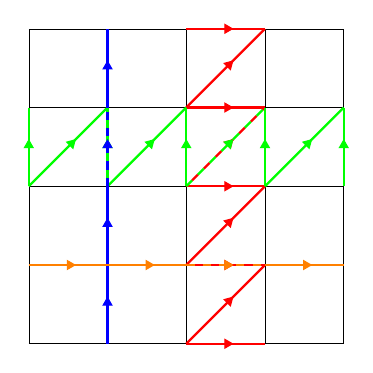
\begin{tikzpicture}
    \draw[step=1cm,black,very thin] (0,0) grid (4,4);
    \begin{scope}[red, thick, decoration={markings, mark=at position 0.6 with {\arrow[scale=0.5]{triangle 60}}}]
        \draw[postaction={decorate}] (2,0) -- (3,0);
        \draw[postaction={decorate},dashed,shorten <=3] (2,1) -- (3,1);
        \draw[postaction={decorate}] (2,2) -- (3,2); 
        \draw[postaction={decorate}] (2,3) -- (3,3);
        \draw[postaction={decorate}] (2,4) -- (3,4);

        \draw[postaction={decorate}] (2,0) -- (3,1);
        \draw[postaction={decorate}] (2,1) -- (3,2);
        \draw[postaction={decorate},dashed,shorten <=3] (2,2) -- (3,3);
        \draw[postaction={decorate}] (2,3) -- (3,4);
    \end{scope}
    \begin{scope}[green, thick, decoration={markings, mark=at position 0.6 with {\arrow[scale=0.5]{triangle 60}}}]
        \draw[postaction={decorate}] (0,2) -- (0,3);
        \draw[postaction={decorate},dashed,shorten <=3] (1,2) -- (1,3);
        \draw[postaction={decorate}] (2,2) -- (2,3); 
        \draw[postaction={decorate}] (3,2) -- (3,3);
        \draw[postaction={decorate}] (4,2) -- (4,3);

        \draw[postaction={decorate}] (0,2) -- (1,3);
        \draw[postaction={decorate}] (1,2) -- (2,3);
        \draw[postaction={decorate},dashed] (2,2) -- (3,3);
        \draw[postaction={decorate}] (3,2) -- (4,3);
    \end{scope}

    \begin{scope}[blue, thick, decoration={markings, mark=at position 0.6 with {\arrow[scale=0.5]{triangle 60}}}]
        \draw[postaction={decorate}] (1,0) -- (1,1);
        \draw[postaction={decorate}] (1,1) -- (1,2);
        \draw[dashed,postaction={decorate}] (1,2) -- (1,3);
        \draw[postaction={decorate}] (1,3) -- (1,4);
    \end{scope}
    \begin{scope}[orange, thick, decoration={markings, mark=at position 0.6 with {\arrow[scale=0.5]{triangle 60}}}]
        \draw[postaction={decorate}] (0,1) -- (1,1);
        \draw[postaction={decorate}] (1,1) -- (2,1);
        \draw[postaction={decorate},dashed] (2,1) -- (3,1);
        \draw[postaction={decorate}] (3,1) -- (4,1);
    \end{scope}
\end{tikzpicture} \end{figure}

\begin{example}
    Consider the 2-torus $\bbT^2$. Define a $\Delta$-complex structure on $\bbT^2$ as in the diagram (with appropriate orientations on the simplices) {\color{red} put diagram here}. Define a function $\phi$ on the edges (1-simplices) of the $\Delta$-complex by taking a red edge to $1$ and all other edges to $0$. As usual, $\phi$ extends uniquely to a cochain which we also denote by $\phi \in C^1_\Delta(\bbT^2;\bbZ)$. Let's show that $\phi$ is a cocycle. To do this, we just need to check $\delta\phi(\sigma) = 0$ for all faces $\sigma \in C_2^\Delta(\bbT^2)$. If $\sigma$ is a face whose boundary does not contain a red edge, then clearly $\delta\phi(\sigma) = 0$. On the other hand, if $\sigma$ is a face with boundary, then $\sigma$ can be either an upper edge, or a lower edge {\color{red} put diagram here}. If $\sigma$ is an upper edge, then $\partial\sigma = a - c + b$, so
    \begin{equation}
        \delta\phi(\sigma) = \phi(\partial\sigma) = \phi(a) - \phi(c) + \phi(b) = 0 - 1 + 1 = 0.
    \end{equation}
    The calculation for a lower edge is similar.

    Now, $\phi$ is not a coboundary. Indeed, suppose it were, and let $\eta \in C_\Delta^1(\bbT^2;\bbZ)$ be such that $\delta\eta = \phi$. Then $\phi(e) = \eta(\partial e) = \eta(v_1) - \eta(v_0)$. Consider the blue 1-chain $c = c_1 + c_2 + c_3 + c_4$ in the diagram, which has boundary $\partial c = 0$, so $\phi(c) = \eta(0) = 0$. However, we also have $\phi(c_3) = 1$ by definition of $\phi$, so $\phi(c) = 1$. Contradiction. This shows that $[\phi]$ is a nonzero element of $H_\Delta^1(\bbT^2;\bbZ) \cong H^1(\bbT^2;\bbZ)$.

    By the universal coefficient theorem,
    \begin{equation}
        H^1(\bbT^2;\bbZ) \cong \Ext(H_0(\bbT^2),\bbZ) \oplus \Hom(H_1(\bbT^2),\bbZ) \cong 0 \oplus \Hom(\bbZ^2,\bbZ) \cong \bbZ^2.
    \end{equation}
    Let $\psi \in C^1_\Delta(\bbT^2;\bbZ)$ be the green cochain in the diagram. As above, $\psi$ is a cocycle but not a coboundary. Let's show that $[\phi]$ and $[\psi]$ are a basis for $H^1_\Delta(\bbT^2;\bbZ)$, and hence are a basis for $H^1(\bbT^2;\bbZ)$. For linear independence, suppose $a,b \in \bbZ$ are such that $a[\phi] + b[\psi] = 0$. That is, $a\phi + b\psi = \delta\eta$ for some $\eta \in C^0_\Delta(\bbT^2;\bbZ)$. Let $c$ be the blue 1-chain as before, and let $d$ be the purple 1-chain. A calculation then gives $a = a\phi(c) + b\psi(c) = \eta(\partial c) = 0$, and $b = a\phi(d) + b\psi(d) = \eta(\partial d) = 0$. On the other hand, to show $[\phi]$ and $[\psi]$ are generators for the cohomology group, first note that $[c]$ and $[d]$ are generators for the homology group $H_1^\Delta(\bbT^2)$. Fix $[\mu] \in H^1_\Delta(\bbT^2;\bbZ)$. Set $a = \mu(c)$, and $b = \mu(d)$, and let $e \in C_1^\Delta(\bbT^2)$ be a 1-chain. Then $e = \alpha c + \beta d + \partial f$ for some 2-chain $f$. We then calculate 
    \begin{equation}
        \mu(e) = \alpha \mu(c) + \beta \mu(d) + \mu(\partial f) 
               = (a\phi + b\psi)(\alpha c + \beta d) 
               = (a\phi + b\psi)(e),
    \end{equation}
    as required.

    Let $v \in C_0^\Delta(\bbT^2)$ be some vertex. Define $v^* \in C^0_\Delta(\bbT^2;\bbZ)$ by $v^*(w) = 1$ if $v = w$, $v^*(w) = 0$ otherwise. The coboundary $\delta v^* \in C^1_\Delta(\bbT^2;\bbZ)$ of $v^*$ is given by the diagram to the right, where $\delta v^*$ associates $+1$ to a red edge, and $-1$ to a blue edge. Note how $\delta$ acts as a kind of ``gradient'': edges coming into $v$ are positive, edges leaving $v$ are negative.
\end{example}

Let's now translate some results in homology to results in cohomology. First, recall if $X$ is a topological space, then its \textit{reduced homology} is the homology of the augmented chain complex 
\begin{equation} 
    \widetilde{C}_* : 
    \begin{tikzcd}
        \cdots \arrow[r] & C_2(X) \arrow[r] & C_1(X) \arrow[r] & C_0(X) \arrow[r,"\epsilon"] & \bbZ \arrow[r] & 0,
    \end{tikzcd}
\end{equation}
where $\epsilon$ is given by $\epsilon(\sigma) = 1$ for $\sigma$ a 0-simplex. We dualize this simplex to obtain $\widetilde{C}^*$, whose cohomology groups are the \textit{reduced cohomology groups} $\widetilde{H}^k(X;G)$. This definition works for the simplicial case as well.

Next, let $(X,A)$ be a pair. Recall the long exact sequence in homology for a pair:
\begin{equation} \begin{tikzcd}
    \cdots \arrow[r] & H_k(A)     \arrow[r, "i_*"] & H_k(X)     \arrow[r, "j_*"] & H_k(X,A)     \arrow[dll, out=355, in=175, "\partial" above] &        \\
                     & H_{k-1}(A) \arrow[r, "i_*"] & H_{k-1}(X) \arrow[r, "j_*"] & H_{k-1}(X,A) \arrow[r]                                      & \cdots 
\end{tikzcd} \end{equation}
Here, the maps $i_*$ and $j_*$ are induced from the respective maps in the short exact sequence of chain complexes 
\begin{equation} \begin{tikzcd} \label{eq:sesForAPair}
    0 \arrow[r] & C_*(A) \arrow[r,"i_\#"] & C_*(X) \arrow[r,"j"] & C_*(X,A) \arrow[r] & 0
\end{tikzcd} \end{equation}
In particular, $j$ is the quotient map (recall $C_k(X,A) := C_k(X)/C_k(A)$), and $i_\#$ is induced from the inclusion $i \colon A \hookrightarrow X$. We can then dualize (\ref{eq:sesForAPair}) to obtain 
\begin{equation} \begin{tikzcd} \label{eq:dualsesForAPair}
    0 & C^*(A;G) \arrow[l]  & C^*(X;G) \arrow[l,"i^\#" above] & C^*(X,A;G) \arrow[l,"j^\#" above] & 0 \arrow[l]
\end{tikzcd} \end{equation}
Note that $C_k(X,A)$ is a free group for all $k$. Indeed, let $S \subseteq C_k(X)$ be the set of all simplices whose image lies in $X \setminus A$. Then $\set{\sigma + C_k(A) : \sigma \in S}$ is a basis for $C_k(X,A)$. A simple diagram chase proves the following lemma:
\begin{lemma}
    Let 
    \begin{equation} \begin{tikzcd}
        0 \arrow[r] & A \arrow[r] & B \arrow[r] & C \arrow[r] & 0
    \end{tikzcd} \end{equation}
    be a split short exact sequence. Then the dual sequence 
    \begin{equation} \begin{tikzcd}
        0 & A^* \arrow[l] & B^* \arrow[l] & C^* \arrow[l] & 0 \arrow[l]
    \end{tikzcd} \end{equation}
    is also split and short exact.
\end{lemma}
With this lemma, we see that (\ref{eq:dualsesForAPair}) is a short exact sequence of cochain complexes. By the zigzag lemma (more precisely, its dual statement for cochain complexes), we obtain the long exact sequence for a pair in cohomology:
\begin{equation} \begin{tikzcd}
    \cdots & H^{k+1}(A;G) \arrow[l]                                 & H^{k+1}(X;G) \arrow[l,"i^*" above] & H^{k+1}(X,A;G) \arrow[l,"j^*" above] &                  \\
           & H^k(A;G)     \arrow[urr,out=175,in=355,"\delta" above] & H^k(X;G)     \arrow[l,"i^*" above] & H^k(X,A;G)     \arrow[l,"j^*" above] & \cdots \arrow[l] 
\end{tikzcd} \end{equation}
More generally, there is a long exact sequence in cohomology coming from the short exact sequence for a triple $(X,A,B)$:
\begin{equation} \begin{tikzcd}
    0 \arrow[r] & C_*(A,B) \arrow[r] & C_*(X,B) \arrow[r] & C_*(X,A) \arrow[r] & 0
\end{tikzcd} \end{equation}

One might ask if there is a connection between the connecting homomorphisms $\delta \colon H^k(A;G) \to H^{k+1}(X,A;G)$ and $\partial \colon H_k(X,A) \to H_{k-1}(A)$. Indeed there is. In fact, the following diagram commutes:
\begin{equation} \begin{tikzcd}
    H^k(A;G)       \arrow[r,"\delta"] \arrow[d,"h"] & H^{k+1}(X,A;G) \arrow[d,"h"] \\
    \Hom(H_k(A),G) \arrow[r,"\partial^*"]           & \Hom(H_{k+1(X,A)},G)
\end{tikzcd} \end{equation}
where $h$ is the map in the universal coefficient theorem. To see this, recall $\partial$ is given by $\partial[z]_{H_{k+1}(X,A)} = [\partial z]_{H_k(A)}$, and $\delta$ is given by $\delta[\alpha]_{H^k(A;G)} = [\delta\alpha]_{H^{k+1}(X,A;G)}$. The rest is easy.




\chapter{The Cohomology Ring}
\section{Cup Products}
In the following, all rings have multiplicative identity.

Let $X$ be a topological space, and $R$ a ring. Choose $\phi \in C^i(X;R)$ and $\psi \in C^j(X;R)$. Given a simplex $\sigma \in C_{i+j}(X)$, define 
\begin{equation}
    (\phi \smile \psi)(\sigma) := \phi(\sigma \vert [v_0,\dots,v_i]) \psi(\sigma \vert [v_i,\dots,v_{i+j}]).
\end{equation}
The \textit{cup product} $\phi \smile \psi \in C^{i+j}(X;R)$ is then defined by extending this linearly to $(i+j)$-chains. The same definition also gives a cup product $C_\Delta^i(X;R) \times C_\Delta^j(X;R) \overset{\smile}{\to} C_\Delta^{i+j}(X;R)$ whenever $X$ has a $\Delta$-complex structure.
\begin{example}
    Consider the 2-torus $\bbT^2$ with the usual $\Delta$-complex structure {\color{red} draw it}. For a simplex $\sigma \in C_k^\Delta(\bbT^2)$, we define $\sigma^* \in C^k_\Delta(\bbT^2;\bbZ)$ by $\sigma^*(\tau) = 1$ if $\tau = \sigma$ and $0$ otherwise. The only interesting cup product is $C^1_\Delta(\bbT^2;\bbZ) \times C^1_\Delta(\bbT^2;\bbZ) \to C^2_\Delta(\bbT^2;\bbZ)$. Let's calculate one. For $a^*$ and $b^*$,
    \begin{equation} \begin{aligned}
        (a^* \smile b^*)(U) &= a^*(U \vert [v_0,v_1]) b^*(U \vert [v_1,v_2]) = a^*(b) b^*(a) = 0, \\
        (a^* \smile b^*)(L) &= a^*(L \vert [v_0,v_1]) b^*(L \vert [v_1,v_2]) = a^*(a) b^*(b) = 1.
    \end{aligned} \end{equation}
    So $a^* \smile b^* = L^*$. This example shows the cup product is not commutative in general. Inded, the same calculation as above shows $b^* \smile a^* = U^*$.
\end{example}

The following three properties of the cup product are easy to check.
\begin{lemma}
    The cup product is $R$-bilinear and associative, and it has identity $\epsilon \in C^0(X;R)$, defined by $\epsilon\parens{ \sum_{i=1}^m a_i \sigma_i } = \sum_{i=1}^m a_i$.
\end{lemma}
Moreover, let $f \colon C_*(X) \to C_*(Y)$ be a chain map. Fix a simplex $\sigma \in C_{i+j}(X)$ and cochains $\phi \in C^i(X;R)$, $\psi \in C^j(X;R)$. Then 
\begin{equation} \begin{aligned}
    f^\#(\phi \smile \psi)(\sigma) &= (\phi \smile \psi)(f(\sigma)) \\
                                   &= \phi(f(\sigma \vert [v_0,\dots,v_i])) \psi(f(\sigma \vert [v_i,\dots,v_{i+j}])) \\
                                   &= (f^\# \phi \smile f^\# \psi)(\sigma).
\end{aligned} \end{equation}
That is, $f^\#(\phi \smile \psi) = f^\# \phi \smile f^\# \psi$.

We would like to show the cup product gives a product on cohomology and not just on cochains. To do this, we need the following ``Leibniz rule'' for the cup product.
\begin{lemma}
    Let $\phi \in C^i(X;R)$ and $\psi \in C^j(X;R)$. Then 
    \begin{equation}
        \delta(\phi \smile \psi) = \delta\phi \smile \psi + (-1)^i \phi \smile \delta\psi.
    \end{equation}
\end{lemma}
\begin{proof}
    Write $n = i + j$, and fix a simplex $\sigma \in C_{n+1}(X)$. Then 
    \begin{equation} \begin{aligned}
        \partial\sigma &= \sum_{k=0}^{n+1} (-1)^k \sigma \vert [v_0,\dots,\widehat{v_k},\dots,v_{n+1}]\\
                       &= \sum_{k=0}^i (-1)^k \sigma \vert [v_0,\dots,\widehat{v_k},\dots,v_i,\dots,v_{n+1}] \\
                       &\quad + (-1)^{i} \sum_{k=1}^{j+1} (-1)^k \sigma \vert [v_0,\dots,v_i,\dots,\widehat{v_{k+i}},\dots,v_{n+1}] \\
                       &=: S + (-1)^i T.
    \end{aligned} \end{equation}
    Now,
    \begin{equation} \begin{aligned}
        (\phi \smile \psi)(S) &= \sum_{k=0}^i (-1)^k \phi(\sigma \vert [v_0,\dots,\widehat{v_k},\dots,v_{i+1}]) 
                                                     \psi(\sigma \vert [v_{i+1},\dots,v_{n+1}]) \\
                              &= (\phi(\partial s) - (-1)^{i+1} \phi(\sigma \vert [v_0,\dots,v_i])) \psi(\sigma \vert [v_{i+1},\dots,v_{n+1}]) \\
                              &= (\delta\phi \smile \psi)(\sigma) + (-1)^i \phi(\sigma \vert [v_0,\dots,v_i]) \psi(\sigma \vert [v_{i+1},\dots,v_{n+1}]),
    \end{aligned} \end{equation}
    where $s = \sigma \vert [v_0,\dots,v_{i+1}]$. On the other hand,
    \begin{equation} \begin{aligned}
        (\phi \smile \psi)(T) &= \sum_{k=1}^{j+1} (-1)^k \phi(\sigma \vert [v_0,\dots,v_i]) 
                                                         \psi(\sigma \vert [v_i,\dots,\widehat{v_{k+i}},\dots,v_{n+1}]) \\
                              &= \phi(\sigma \vert [v_0,\dots,v_i]) (\psi(\partial t) - \psi(\sigma \vert [v_{i+1},\dots,v_{n+1}])) \\
                              &= (\phi \smile \delta\psi)(\sigma) - \phi(\sigma \vert [v_0,\dots,v_i]) \psi(\sigma \vert [v_{i+1},\dots,v_{n+1}]),
    \end{aligned} \end{equation}
    where $t = \sigma \vert [v_i,\dots,v_{n+1}]$. Combining the above three equations and using $\delta(\phi \smile \psi)(\sigma) = (\phi \smile \psi)(\partial\sigma)$ gives the desired result.
\end{proof}

The Leibniz rule means we have a well-defined cup product on cohomology. To show this, let $\phi \in Z^i(X;R)$ and $\psi \in Z^j(X;R)$ be cocycles. Then
\begin{equation}
    \delta(\phi \smile \psi) = \delta\phi \smile \psi + (-1)^i \phi \smile \delta\psi = 0,
\end{equation}
so $\phi \smile \psi$ is an $(i+j)$-cocycle, and we can take its cohomology $[\phi \smile \psi] \in H^{i+j}(X;R)$. Define $[\phi] \smile [\psi] := [\phi \smile \psi]$. To show this is well-defined, let $\phi' \in Z^i(X;R)$ be such that $[\phi] = [\phi']$. Then $\phi' = \phi + \delta\eta$ for some $\eta \in C^{i-1}(X;R)$, so $[\phi' \smile \psi] = [\phi \smile \psi] + [\delta\eta \smile \psi]$. However, by the Leibniz rule, we know $\delta\eta \smile \psi = \delta(\eta \smile \psi) - (-1)^{i-1}(\eta \smile \delta\psi) = \delta(\eta \smile \psi)$ since $\psi$ is a cocycle. Hence $\delta\eta \smile \psi$ is a coboundary, and so $[\delta\eta \smile \psi] = 0$. It follows that $[\phi' \smile \psi] = [\phi \smile \psi]$. The same is true for $\psi$, so the cup product on cohomology is well defined.

As for the cup product on cocycles, the cup product on cohomology is $R$-bilinear, associative, and has $[\epsilon]$ as its identity. Moreover, induced homomorphisms distribute over the cup product, in the sense that if $f \colon C_*(X) \to C_*(Y)$ is a chain map, then $f^*[\phi \smile \psi] = f^*[\phi] \smile f^*[\psi]$.

We will now spend some time calculating the cohomology groups and some cup products in a number of spaces.
\begin{example}
    Let $X$ be a discrete space. {\color{red} draw a picture of a discrete space} Its chain groups are then isomorphic to $\oplus_{x \in X} \bbZ$ in dimension $0$, and $0$ in every other dimension, so the homology of $X$ is $H_0(X) \cong \oplus_{x \in X} \bbZ$. Taking the dual with coefficients in $R$, we have the cochain complex $0 \leftarrow \Hom(\oplus_{x \in X}, R) \leftarrow 0$. However, $\Hom(\oplus_{x \in X}, R) \cong \prod_{x \in X} R$, so $H^0(X;R) \cong \prod_{x \in X} R$, which is the set of functions $X \to R$.
\end{example}
\begin{example} \label{eg:graphs}
    Let $X$ be a graph. {\color{red} draw a graph} That is, a one-dimensional $\Delta$-complex. Then $C_0^\Delta(X)$ is the free abelian group on the set $X^0$ of vertices in $X$, whose dual is $C^0_\Delta(X;R) \cong \prod_{x \in X^0} R$. Note that $\phi \in C^0_\Delta(X;R)$ is a cocycle if and only if $\delta\phi(e) = \phi(v_1 - v_0) = 0$ for all edges $e \in X^1$ with boundary $v_1 - v_0$. In particular, if $v, w \in X^0$ lie in the same component of $X$, they are connected by a path of edges, so $\phi$ must be constant on components of $X$. Conversely, if $\phi$ is constant on components of $X$, then $\phi$ is a cocycle. It follows that $H^0(X;R) \cong Z^0_\Delta(X;R) \cong \prod_{A \in \scrA} R$, where $\scrA$ is the set of components in $X$.

    In order to calculate $H^1(X;R)$, we just need to calculate $B^1_\Delta(X;R)$. Without loss of generality, $X$ is connected. Suppose $\phi = \delta\psi \in C^1_\Delta(X;R)$ is a coboundary. Given a directed loop of edges $e_1,\dots,e_n$ based at $v \in X^0$, we have 
    \begin{equation}
        \phi\parens{ \sum_{i=1}^n e_i } = \psi(v) - \psi(v) = 0,
    \end{equation}
    so $\phi$ vanishes on directed loops in $X$. Conversely, suppose $\phi$ vanishes on directed loops on $X$. Fix a basepoint $v_0 \in C_0^\Delta(X)$, and define $\psi \in C^0_\Delta(X;R)$ by $\psi(v) = \sum_{i=1}^n \phi(e_i)$, where $e_1,\dots,e_n$ is a directed path in $X^1$ from $v_0$ to $v$. This is well-defined, since if $e_1',\dots,e_m'$ is another directed path from $v_0$ to $v$, then $e_1,\dots,e_n,-e_m',\dots,-e_1'$ is a directed loop at $v_0$, so 
    \begin{equation}
        0 = \phi(\sum_{i=1}^n e_i - \sum_{i=1}^m e_i') = \sum_{i=1}^n \phi(e_i) - \sum_{i=1}^m \phi(e_i').
    \end{equation}
    Furthermore, for any edge $e \in C_1^\Delta(X)$ with boundary $w - v$ let $e_1,\dots,e_n$ be a directed path from $v_0$ to $w$, and $e_1',\dots,e_m'$ a directed path from $v_0$ to $v$. Then $e_1',\dots,e_m',e,-e_n,\dots,-e_1$ is a loop at $v_0$, so we have 
    \begin{equation}
        \delta\psi(e) = \psi(w) - \psi(v) = \sum_{i=1}^n \phi(e_i) - \sum_{i=1}^m \phi(e_i') = \phi(e).
    \end{equation}
    Thus $\phi$ is a coboundary. It follows that $B^1_\Delta(X;R)$ are the elements of $C^1_\Delta(X;R)$ vanishing on directed loops in $X$.

    The homology of $X$ is isomorphic to the free group on the set of edges in $X \setminus T$, where $T$ is a spanning tree for $X$. By the universal coefficient theorem, $H^1(X;R) \cong \Hom(H_1(X),R) \cong \prod_{e \in C_1^\Delta(X \setminus T)} R$.

    Note that since cohomology exists only in dimensions 0 and 1, the cup product structure on $X$ is uninteresting.
\end{example}

Having discussed 0- and 1-dimensional objects, let's consider surfaces. By the surface classification theorem, every surface (potentially with boundary) is homeomorphic to some 
\begin{equation}
    S_{g,b,c} := S^2 \# \parens{ \consum_{i=1}^g \bbT^2 } \# \parens{ \consum_{i=1}^b B } \# \parens{ \consum_{i=1}^c \bbR\bbP^2 },
\end{equation}
where $B \subseteq \bbR^2$ is the closed unit ball. In particular, every surface with $b = 0$ is given by a polygon, modulo an equivalence relation on the edges of its boundary (for example, $\bbT^2$ is given by the unit square, modulo the equivalence relation identifying opposite edges with each other). This can be expressed as a ``polygonal presentation'' of the form $\left\langle S \middle\vert R \right\rangle$, where $S$ is some finite set, and $R$ some relations on $S$. For example, $\bbT^2$ is given by the polygonal presentation $\left\langle a,b \middle\vert aba^{-1}b^{-1} \right\rangle$. We won't delve deep into this - see {\bf [Lee]}. What is important is that if $M$ is a surface with $b = 0$ given by a polygonal presentation, taking a connected sum with a disk is equivalent to cutting a hole in the polygon. This polygon minus a hole deformation retracts onto its boundary, so it follows that $M \# B$ is homotopy equivalent to a graph. Similary, $M \# B \# B$ is equivalent to cutting two holes in a polygon hence deformation retracts onto a graph, etc. The surfaces $S_{g,b,c}$ with $b \geq 1$ are therefore homotopy equivalent to graphs, whose cohomology has been dealt with in example \ref{eg:graphs}.

Next, we state without proof that $\bbT^2 \# \bbRP^2 \cong \bbRP^2 \# \bbRP^2 \# \bbRP^2$ (again, see {\bf [Lee]}). Recalling that $S^2 \# M \cong M$ for any surface $M$, we see that the only interesting surfaces are the sphere $S^2$, the \textit{orientable surface of genus} $g$ 
\begin{equation}
    M_g := S_{g,0,0} = \consum_{i=1}^g \bbT^2,
\end{equation}
and the \textit{nonorientable surface of nonorientable genus} $c$ 
\begin{equation}
    N_c := S_{0,0,c} = \consum_{i=1}^c \bbRP^2.
\end{equation}
We will consider the homology of these surfaces in turn.

\begin{figure} 
    \centering
    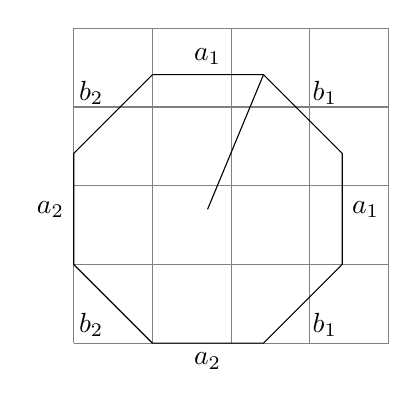
\begin{tikzpicture}
        \draw[gray] (0,0) grid (4,4);

        \draw (0,1) -- (0.5,0.5) node[below left] {$b_2$} -- (1,0) -- (1.7,0) node[below] {$a_2$} -- (2.41,0) 
                    -- (2.91,0.5) node[below right] {$b_1$} -- (3.41,1) -- (3.41,1.7) node[right] {$a_1$} -- (3.41,2.41) 
                    -- (2.91,2.91) node[above right] {$b_1$} -- (2.41,3.41) -- (1.7,3.41) node[above] {$a_1$} -- (1,3.41) 
                    -- (0.5,2.91) node[above left] {$b_2$} -- (0,2.41) -- (0,1.7) node[left] {$a_2$} -- (0,1);

        \draw (1.7,1.7) -- (2.41,3.41);
    \end{tikzpicture}
\end{figure}
\begin{example} \label{eg:orientableSurface}
    First, consider the orientable surface $M_g$. This surface has polygonal presentation $\left\langle a_1,b_1,\dots,a_g,b_g \middle\vert [a_1,b_1] \cdots [a_g,b_g] \right\rangle$, where $[a_i,b_i] := a_i b_i a_i^{-1} b_i^{-1}$ is the \textit{commutator} of $a_i$ and $b_i$. Equip $M_g$ considered as a $4g$-gon with appropriate identifications with its usual $\Delta$-complex structure {\color{red} draw picture}.
    Now by, say, cellular homology, the edges $a_i$ and $b_i$ form a basis for the homology group $H_1(M_g)$. In particular, $H_1(M_g) \cong \bbZ^{2g}$. As usual, $H_0(M_g) \cong \bbZ$, and $H_2(M_g) \cong \bbZ$. By the universal coefficient theorem, we see $h \colon H^1(M_g) \to \Hom(H_1(M_g),R)$ is an isomorphism. Write $\alpha_i = [a_i]^* \in \Hom(H_1(M_g),R)$. In order to calculate cup products $H^1(M_g;R) \times H^1(M_g;R) \to H^2(M_g;R)$, we need to find a cocycle $\phi_i \in C^1_\Delta(M_g;R)$ with $h[\phi_i] = \alpha_i$. Since we require
    \begin{equation}
        \phi_i(a_j) = h[\phi_i][a_j] = \alpha_i[a_j] = \delta_{ij},
    \end{equation}
    we just need to specify the value of $\phi_i$ on the remaining 1-simplices $x_1,y_1,\overline{x}_1,\overline{y}_1,\dots,x_g,y_g,\overline{x}_g,\overline{y}_g$. Now, for $\phi_i$ to be a cocycle, we need $\delta\phi_i = 0$. In particular, we have
    \begin{equation} \begin{aligned}
        0 &= \delta\phi_i(\sigma_j) = \phi_i(\partial \sigma_j) = \phi_i(x_j) + \phi(a_j) - \phi(y_j) \\
        0 &= \delta\phi_i(\tau_j)   = \phi_i(\partial\tau_j)    = \phi_i(y_j) + \phi(b_j) - \phi(\overline{x}_j) \\
        0 &= \delta\phi_i(\overline{\sigma}_j) = \phi_i(\partial\overline{\sigma}_j) = - \phi_i(\overline{x}_j) + \phi_i(a_j) + \phi_i(\overline{y}_j) \\
        0 &= \delta\phi_i(\overline{\tau}_j) = \phi_i(\partial\overline{\tau}_j) = - \phi_i(\overline{y}_j) + \phi_i(b_j) + \phi_i(x_{j+1})
    \end{aligned} \end{equation}
    where addition of the indices is taken mod $g$. It follows that $\phi_i$ is determined uniquely by its value on $x_1$. Take $\phi_i(x_1) = 0$. Consequently, $\phi_i$ is well-defined since the equations show $\phi_i(x_j) = \phi_i(\overline{y}_j) = 0$ for all $j$, and $\phi_i(y_j) = \phi_i(\overline{x}_j) =  \delta_{ij}$. By construction, $\phi$ is a cocycle. Finally, note that $h[\phi_i] = \alpha_i$ also by construction.

    We now have enough information to compute $\phi_i \smile \phi_j$. Consider first $i = j$. In this case, 
    \begin{equation} \begin{aligned}
        (\phi_i \smile \phi_i)(\sigma_j) &= \phi_i(x_j) \phi_i(a_j) = 0; \\
        (\phi_i \smile \phi_i)(\tau_j)   &= \phi_i(y_j) \phi_i(b_j) = 0; \\
        (\phi_i \smile \phi_i)(\overline{\sigma}_j) &= \phi_i(\overline{y}_j) \phi_i(a_j) = 0; \\
        (\phi_i \smile \phi_i)(\overline{\tau}_j) &= \phi_i(x_{j+1}) \phi_i(b_j) = 0.
    \end{aligned} \end{equation}
    So $\phi_i \smile \phi_i = 0$. In terms of homology, $\alpha_i \smile \alpha_i = 0$. A similar calculation shows us $\phi_i \smile \phi_j = 0$ for $i \neq j$.

    The same construction gives us cocycles $\psi_i$ with $h[\psi_i] = \beta_i$. In this case, $\psi_i(x_j) = \psi_i(y_j) = 0$ for all $j$, and $\psi_i(\overline{x}_j) = \psi_i(\overline{y}_j) = \delta_{ij}$. As above $\psi_i \smile \psi_j = 0$ for all $i,j$. Let's calculate $\phi_i \smile \psi_j$:
    \begin{equation} \begin{aligned}
        (\phi_i \smile \psi_j)(\sigma_k) &= \phi_i(x_k) \psi_j(a_k) = 0; \\
        (\phi_i \smile \psi_j)(\tau_k) &= \phi_i(y_k) \psi_j(b_k) = \delta_{ij} \delta_{jk}; \\
        (\phi_i \smile \psi_j)(\overline{\sigma}_k) &= \phi_i(\overline{y}_k) \psi_j(a_k) = 0; \\
        (\phi_i \smile \psi_j)(\overline{\tau}_k) &= \phi_i(x_{j+1}) \psi_j(b_j) = 0. \\
    \end{aligned} \end{equation}
    It follows that $\phi_i \smile \psi_i = \tau_i^*$, and $\phi_i \smile \psi_j = 0$ for $i \neq j$. Similarly, we may calculate $\psi_i \smile \phi_i = \overline{\sigma}_i^*$.

    Again by the universal coefficient theorem, $H^2(M_g;R) \cong \Hom(H_2(M_g),R)$. A generator for $H_2(M_g)$ is given by the 2-chain 
    \begin{equation}
        z = \sum_{i=1}^g \sigma_i + \tau_i - \overline{\sigma}_i - \overline{\tau}_i.
    \end{equation}
    Write $\gamma = h^{-1}[z]^*$. It follows by our calculations that $\alpha_i \smile \beta_i = \gamma = -\beta_i \smile \alpha_i$.

    The $\alpha_i$ and $\beta_i$ have a nice geometric interpretation: draw an arc from the positive orientation $a_i$ to the negative orientation $a_i$. Then $\alpha_i(\sigma)$ counts how many times $\sigma$ intersects this arc. Similar for $\beta_i$.
\end{example}
\begin{example}
    Now we move on to the nonorientable surface $N_c$. This surface has polygonal presentation $\left\langle a_1,\dots,a_c \middle\vert a_1 a_1 \cdots a_c a_c \right\rangle$. Equip it with the usual $\Delta$-complex structure {\color{red} draw it}. As for $M_g$, the edges $a_i$ form a basis for $H_1(N_c)$.

\end{example} 

\begin{theorem}
    Let $X$ be a topological space and $R$ a commutative ring. Choose $\alpha \in H^k(X;R)$ and $\beta \in H^l(X;R)$. Then 
    \begin{equation}
        \alpha \smile \beta = (-1)^{kl} \beta \smile \alpha. 
    \end{equation}
\end{theorem}


\section{The Cohomology Ring}

In this section, we fix a commutative ring $R$. An $R$-module $M$ is an abelian group equipped with a scalar multiplication $R \times M \to M$ satisfying
\begin{itemize}
    \item $r(x+y) = rx + ry$,
    \item $(r+s)x = rx + sx$,
    \item $(rs)x = r(sx)$,
    \item $1_R x = x$
\end{itemize}
for all $r,s \in R$ and $x,y \in M$. An $R$-algebra $A$ is an $R$-module equipped with a multiplication $A \times A \to A$ making $A$ into a ring, and such that 
\begin{equation}
    r(xy) = (rx)y = x(ry)
\end{equation}
for all $r \in R$ and $x,y \in A$. 
\begin{example}
    Polynomial rings $R[x_1,\dots,x_n]$ and their quotients are algebras over $R$. Of course, the quotient algebra $R[x]/(x^2)$ is isomorphic as an $R$-module to $R \oplus R$.
\end{example}

An $R$-algebra $A$ is \textit{graded} if it can be decomposed as a direct sum $\bigoplus_{k=0}^\infty A_k$, where each $A_k$ is a submodule of $A$, and multiplication satisfies $A_k A_l \subseteq A_{k+l}$.
\begin{example}
    The polynomial algebra $R[x_1,\dots,x_n]$ is a graded $R$-algebra, whose degree $k$ component is the submodule generated by the monomials of degree $k$.
\end{example}

Given a topological space $X$, its \textit{cohomology ring} $H^*(X;R)$ is the graded $R$-algebra with multiplication given by the cup product, and whose degree $k$ component is $H^k(X;R)$.
\begin{example}
    In example \ref{eg:orientableSurface}, we calculated the cohomology ring of $\bbT^2 = M_1$ to be the exterior algebra $\Lambda[\alpha_1,\beta_1]$.
\end{example}

Given graded $R$-algebras $A$ and $B$, we define their \textit{graded tensor product} $A \otimes_R B$ to be the graded algebra with degree $k$ component
\begin{equation}
    (A \otimes_R B)_k := \bigoplus_{i+j=k} A_i \otimes_R B_j,
\end{equation}
the tensor product being that of $R$-modules, with multiplication given by 
\begin{equation}
    (a \otimes b)(a' \otimes b') := (-1)^{\deg{b}\deg{a'}} aa' \otimes bb'.
\end{equation}

Let $X$ and $Y$ be topological spaces, and consider the projection maps $p_X \colon X \times Y \to X$ and $p_Y \colon X \times Y \to Y$. Apply the cohomology functor to obtain $R$-algebra homomorphisms $p_X^* \colon H^*(X;R) \to H^*(X \times Y;R)$ and $p_Y^* \colon H^*(Y;R) \to H^*(X \times Y;R)$. We define the \textit{cross product} $\times \colon H^*(X;R) \times H^*(Y;R) \to H^*(X \times Y;R)$ by
\begin{equation}
    \alpha \times \beta := p^*_X \alpha \smile p^*_Y \beta.
\end{equation}
This product is evidently bilinear, and also satisfies 
\begin{equation} \begin{aligned}
    (\alpha \times \beta) \smile (\alpha' \times \beta')
    &= p_X^* \alpha \smile p_Y^* \beta \smile p_X^* \alpha' \smile p_Y^* \beta' \\
    &= p_X^* \alpha \smile ( (-1)^{\deg{p_Y^* \beta} \deg{p_X^* \alpha'}} p_X^* \alpha' \smile p_Y^* \beta ) \smile p_Y^* \beta' \\
    &= (-1)^{\deg{\beta} \deg{\alpha'}} (\alpha \smile \alpha') \times (\beta \smile \beta').
\end{aligned} \end{equation}
By the universal property for the graded tensor product, the cross product therefore induces an $R$-algebra homomorphism $\mu \colon H^*(X;R) \otimes_R H^*(Y;R) \to H^*(X \times Y;R)$, which we also call the cross product.
\begin{theorem}[K\"unneth Formula]
    Let $X$ and $Y$ be CW complexes such that $H^k(Y;R)$ is a finitely generated free $R$-module for all $k$. Then $\mu$ is an $R$-algebra isomorphism.
\end{theorem}
There is also a relative version of the K\"unneth formula:
....



\chapter{Poincar\'e Duality}
\section{Manifolds and Orientability}

Throughout this section, fix an $n$-manifold $M$ and a commutative ring $R$. For $B \subseteq M$, we define the \textit{local homology} of $M$ at $B$ to be the groups $H_k(M \vert B;R) := H_k(M,M \setminus B;R)$. Note that if $A \subseteq B \subseteq M$, then $M \setminus B \subseteq M \setminus A$, inducing a map $\psi_{B,A} \colon H_k(M \vert B;R) \to H_k(M \vert A;R)$. It follows that $H(M \vert \cdot;R)$ is a contravariant functor from subsets of $M$ to $R$-modules. If $B$ is an embedded open $n$-ball around $x \in M$, then $M \setminus \set{x} \simeq M \setminus B$. Since $(M,M \setminus B)$ is a good pair, we have $H_k(M \vert B;R) \cong \widetilde{H}_k(M / (M \setminus B) ; R)$. But $M / (M \setminus B) \cong S^n$, so $H_n(M \vert x ; R) \cong H_n(S^n ; R) \cong R$, and $H_k(M \vert x ; R) = 0$ for $k \neq n$.
We will be using the maps $\psi_{B,A}$ constantly from now on. As a shorthand, we write $\psi_x := \psi_{M,x} \colon H_k(M;R) \to H_k(M \vert x;R)$.

Define the fiber bundle $\pi \colon M_R \to M$ by setting $M_R := \set{ (x,\alpha) \in M \times R : \alpha \in H_n(M \vert x ; R) }$. We give $M_R$ a topology by choosing as a subbase the sets 
\begin{equation}
    U(B,I) := \set{ (x,\alpha) \in M_R : x \in B, \alpha \in \psi_{B,x}(I) }
\end{equation} 
for $B \subseteq M$, $I \subseteq R$ open. We call $M_R$ the \textit{local homology bundle} of $M$. {\color{red} check that $M_R$ is a fiber bundle.} An $R$-\textit{orientation} of $M$ is a section $\alpha$ of $M_R$ such that for all $x \in M$, $\alpha_x$ is a unit in $R$ (equivalently, $\alpha_x$ is a generator of the $R$-module $H_n(M \vert x ; R) \cong R$. The manifold $M$ is $R$-\textit{orientable} if it admits an $R$-orientation. We see immediately that any manifold is $\bbZmod{2}$-orientable.
\begin{theorem} \label{thm:HomoOfOrientableMfds}
    Let $M$ be a closed and connected $n$-manifold, and $R$ a commutative ring. Then
    \begin{enumerate}[label={\rm (\arabic*)}]
        \item If $M$ is $R$-orientable, then the map $\psi_x \colon H_n(M;R) \to H_n(M \vert x;R)$ is an isomorphism for all $x \in M$.
        \item If $M$ is $R$-nonorientable, then the above map is injective with image $\set{r \in R : r = -r}$.
        \item For $i > n$, we have $H_i(M;R) = 0$.
    \end{enumerate}
\end{theorem}
An element of $H_n(M;R)$ whose image in $H_n(M \vert x;R)$ is a generator for all $x$ is called a \textit{fundamental class} for $M$, and is usually denoted $[M]$. By the theorem, a closed and $R$-orientable manifold admits a fundamental class. In fact, the converse is true:
suppose $M$ has a fundamental class $[M] \in H_n(M;R)$. Immediately from the definition, we see that $M$ is $R$-orientable. Also, $M$ is compact since the image of any cycle representing $[M]$ must be compact, and so if $x$ were to lie outside this image, then $\psi_x[M] = 0$.

The theorem will following from the following technical lemma:
\begin{lemma}
    Let $M$ be an $n$-manifold and $K \subseteq M$ compact. Then
    \begin{enumerate}[label={\rm (\arabic*)}]
        \item If $\alpha$ is a section of $\pi \colon M_R \to M$, then there is a unique class $\alpha_K \in H_n(M \vert K;R)$ such that $\psi_{K,x}(\alpha_K) = \alpha_x$ for all $x \in K$.
        \item For $i > n$, we have $H_i(M \vert K;R) = 0$.
    \end{enumerate}
\end{lemma}

\begin{proof}[Proof of theorem \ref{thm:HomoOfOrientableMfds}]
    Suppose $M$ is $R$-orientable, and let $\alpha \in \Gamma(M_R)$ be an $R$-orientation. Since $M$ is compact, we may use the above lemma to give us a class $\alpha_M \in H_n(M ; R)$ such that $\psi_x(\alpha_M) = \alpha_x$ for all $x \in M$. So $\alpha_M$ is a fundamental class for $M$. Part (3) of the theorem follows immediately from part (2) of the above lemma.

    Part (2) is what
\end{proof}

\begin{proposition}
    If $M$ is a connected and noncompact $n$-manifolds, then $H_i(M;R) = 0$ for $i \geq n$.
\end{proposition}


\section{Poincar\'e Duality}

Let $X$ be a topological space and $R$ a ring. For $k \geq l$, we define the \textit{cap product} $\frown \colon C_k(X;R) \times C^l(X;R) \to C_{k-l}(X;R)$ by
\begin{equation}
    \sigma \frown \psi := \psi(\sigma \vert [v_0,\dots,v_l]) \sigma \vert [v_l,\dots,v_k].
\end{equation}
Analogous to the Leibniz rule for the cup product, there is a similar rule for the cap product:
\begin{lemma}
    For $k \geq l$, let $\sigma \in C_k(X;R)$ and $\psi \in C^l(X;R)$. Then
    \begin{equation}
        \partial(\sigma \frown \psi) = (-1)^l(\partial \sigma \frown \psi - \sigma \frown \delta\psi).
    \end{equation}
\end{lemma}
Thanks to this lemma, the cap product descends to a cap product on homology $H_k(X;R) \times H^l(X;R) \to H_{k-l}(X;R)$. There is also a relative cap product $H_k(X,A \cup B;R) \times H^l(X,A;R) \to H_{k-l}(X,B;R)$. Finally, the cap product has a decent naturality formula. Namely, for a map $f \colon X \to Y$, we have 
\begin{equation}
    f_\# \sigma \frown \psi = f_\# (\sigma \frown f^\# \psi).
\end{equation}

We can now state Poincar\'e duality.
\begin{theorem}[Poincar\'e Duality]
    Let $M$ be a closed and $R$-orientable $n$-manifold with fundamental class $[M] \in H_n(M;R)$. Then the map $D \colon H^k(M;R) \to H_{n-k}(M;R)$, defined by $D(\alpha) := [M] \frown \alpha$, is an isomorphism for all $k \in \bbN_0$.
\end{theorem}

\begin{example}
    We return to our example of the orientable surface $M_g$ (example \ref{eg:orientableSurface}). Working in simplicial (co)homology and with our notation as before, we saw that a fundamental class for $M_g$ was given by the cycle
    \begin{equation}
        \sum_{i=1}^g \sigma_i + \tau_i - \overline{\sigma}_i - \overline{\tau}_i.
    \end{equation}
    Applying the duality map to the homology classes $\alpha_i, \beta_i \in H^1(M_g;\bbZ)$, we have 
    \begin{equation}
        [M_g] \frown \phi_i = b_i,
    \end{equation}
    and 
    \begin{equation}
        [M_g] \frown \psi_i = -a_i.
    \end{equation}
\end{example}

The proof of Poincar\'e duality is a special case of a more general form of Poincar\'e duality, using what is known as \textit{cohomology with compact supports}. Let $X$ be a topological space and $G$ an abelian group. We define $C_c^i(X;G)$ to be the subgroup of $C^i(X;G)$ consisting of cochains $\phi$ for which there exists a compact set $K \subseteq X$ with $\phi(\sigma) = 0$ for all $\sigma \in C_i(X)$ with support in $X \setminus K$. If $\phi \in C_c^i(X;G)$, then $\delta\phi \in C_c^{i+1}(X;G)$. Indeed, let $K \subseteq X$ be as above, and let $\sigma \in C_{i+1}(X)$ be a simplex with support in $K$. Then the simplices making up $\partial\sigma$ have support in $X \setminus K$, from which it immediately follows that $\delta\phi(\sigma) = \phi(\partial\sigma) = 0$. The cohomology groups of the cochain complex $C_c^i(X;G)$ are denoted $H_c^i(X;G)$, and are called the \textit{cohomology groups with compact supports}.

A more algebraic definition of cohomology with compact supports is possible, and will be important in the proof of Poincar\'e duality. Let $(I,\leq)$ be a \textit{directed set}, i.e. a poset with the property that for any $\alpha,\beta \in I$, there exists $\gamma \in I$ such that $\alpha,\beta \leq \gamma$. A \textit{directed system} is a covariant functor $(I,\leq) \to \textrm{Ab}$. More concretely, a directed system is a family $(G_\alpha)_{\alpha \in I}$ of abelian groups such that for $\alpha \leq \beta$, there exists a homomorphism $f_{\alpha \beta} \colon G_\alpha \to G_\beta$ with the property that if $\alpha \leq \beta \leq \gamma$, then $f_{\beta \gamma} \circ f_{\alpha \beta} = f_{\alpha \gamma}$. The \textit{direct limit} $\varinjlim G_\alpha$ of this system is defined in two equivalent ways: first, let $G = \bigoplus_{\alpha \in I} G_\alpha$, and let $H$ be the subgroup of $G$ generated by elements of the form $a - f_{\alpha\beta}(a)$ for $\alpha \leq \beta$ and $a \in G_\alpha$, naturally regarding each $G_\alpha$ as a subgroup of $G$. We define $\varinjlim G_\alpha := G/H$. 

For the other definition, let $G$ be the set $\coprod_{\alpha \in I} G_\alpha$. Define an equivalence relation on $G$ by saying $a \sim b$ if and only if there exists $\gamma \geq \alpha,\beta$ such that $f_{\alpha\gamma}(a) = f_{\beta\gamma}(b)$ for all $a \in G_\alpha, b \in G_\beta$. That is, if and only if $a$ and $b$ are ``eventually equal'' in the directed system $(G_\alpha)_{\alpha \in I}$. Define a group operation on $G/\sim$ by setting $[a] + [b] := [f_{\alpha\gamma}(a) + f_{\beta\gamma}(b)]$, where $\gamma \geq \alpha,\beta$. This is well-defined, and makes $G/~$ into an abelian group. Define a map $G/~ \to \varinjlim G_\alpha$ by taking $[a]$ to the coset of $a$ in $\varinjlim G_\alpha$. This is also well-defined, is a homomorphism, and has an inverse given by $\sum_i a_i \mapsto \sum_i [a_i]$. We thus identify $G/~$ with $\varinjlim G_\alpha$.

A subset $J$ of a directed set $(I,\leq)$ is called \textit{cofinal} if, for any $\alpha \in I$, there exists $\beta \in J$ with $\alpha \leq \beta$. A consequence of the definition of the direct limit using disjoint unions is that $\varinjlim_{\alpha \in J} G-\alpha \cong \varinjlim_{\alpha \in I} G_\alpha$. Indeed, any $a \in G_\alpha$ is eventually equal to some $f_{\alpha\beta}(a)$, where $\beta \in J$ is such that $\beta \geq \alpha$. In particular, if $\gamma \in I$ is a maximal element, then we can take $J = \set{\gamma}$ to see that $\varinjlim G_\alpha \cong G_\gamma$.

The direct limit satisfies the following property which characterizes the category-theoretic direct limit: given any other abelian group $H$ and a collection of homomorphisms $g_\alpha \colon G_\alpha \to H$ satisfying $g_\alpha = g_\beta \circ f_{\alpha\beta}$ whenever $\alpha \leq \beta$, then there exists a unique homomorphism $g \colon \varinjlim G_\alpha \to H$ such that $g[a] = g_\alpha(a)$ for all $a \in G_\alpha$. In particular, if a topological space $X$ is the union of subspaces $X_\alpha$ (forming a directed set under inclusion), then inclusion induces a homomorphism $\varinjlim H_k(X_\alpha;G) \to H_k(X;G)$. A particular special case is as follows:
\begin{proposition}
    Let $X$ be a topological space given by the union of subspaces $X_\alpha$ with the property that every compact set in $X$ is contained in some $X_\alpha$. Then the homomorphism $\varinjlim H_k(X_\alpha;G) \to H_k(X;G)$ is an isomorphism for each $k$.
\end{proposition}
\begin{proof}
    For surjectivity, let $b \in H_k(X;G)$. Then $b$ is represented by a cycle whose image is compact in $X$, and therefore $b$ lies in some $H_k(X_\alpha;G)$. The equivalence class $[b] \in \varinjlim H_k(X_\alpha;G)$ then gets mapped to $b$. For injectivity, let $a \in H_k(X_\alpha;G)$, and suppose $a = 0$ in $H_k(X;G)$. Then $a$ is represented by a boundary whose image is compact in $X$, implying it is a boundary in some $X_\beta$. Thus $a = 0$ in $H_k(X_\beta;G)$, implying $[a] = [0]$ in $\varinjlim H_k(X_\alpha;G)$.
\end{proof}

Let's now define cohomology with compact supports in terms of direct limits. Let $X$ be a topological space, and consider the directed set consisting of compact subsets of $X$ with inclusion as the relation. Consider the directed system afforded by the covariant functor $H^k(X \vert \cdot;G)$. We claim $\varinjlim H^k(X \vert K ; G) \cong H^k_c(X ; G)$. Indeed, spiddly doodly doo. If $X$ is compact, then the directed set of compact subsets of $X$ has a maximal element, namely $X$, which shows that $H_c^k(X;G) \cong H^k(X;G)$.

\begin{example}
    Let's calculate the cohomology of $\bbR^n$ with compact supports. The collection $(\overline{B(0,r)})_{r > 0}$ is cofinal in the directed set of compact subsets of $\bbR^n$, so it suffices to restrict to this collection. Now,
    \begin{equation}
        H^k(\bbR^n \vert \overline{B(0,r)} ; G) \cong
        \begin{cases}
            G & k = n, \\
            0    & k \neq n.
        \end{cases}
    \end{equation}
    Furthermore, for $r > s$, the map $H^k(\bbR^n \vert \overline{B(0,s)} ; G) \to H^k(\bbR^n \vert \overline{B(0,r)} ; G)$ is an isomorphism. It follows that $H_c^n(\bbR^n ; G) = \varinjlim H^n(\bbR^n \vert K ; G) \cong G$, and $H_c^k(\bbR^n ; G) = 0$ for $k \neq n$.
\end{example}

Using cohomology with compact supports, we can state a duality theorem for noncompact manifolds. First, we need to find out what the duality map is. Let $R$ be a ring, and let $M$ be an $R$-orientable $n$-manifold. Choose an $R$-orientation $\mu \in \Gamma(M_R)$ for $M$. Choose compact sets $K \subseteq L \subseteq M$, and ... 

\begin{theorem}
    The duality map $D_M \colon H^k_c(M;R) \to H^k(M;R)$ is an isomorphism.
\end{theorem}

\begin{corollary}
    A closed $\bbZ$-orientable manifold of odd dimension has Euler characteristic zero.
\end{corollary}
\begin{proof}
    Recall the Euler characteristic of $M$ is defined by $\chi(M) := \sum_{k=0}^n (-1)^k \rank{H_k(M)}$, where $n$ is the dimension of $M$ Suppose now $n$ is odd. Then, for $k = \frac{n+1}{2},\dots,n$, we have $H_k(M) \cong H^{n-k}(M;\bbZ)$. By the universal coefficient theorem, $\rank{H^{n-k}(M;\bbZ)} = \rank{H_{n-k}(M)}$. It follows that
    \begin{equation} \begin{aligned}
        \chi(M) 
        &= \sum_{k=0}^n (-1)^k \rank{H_k(M)} \\
        &= \sum_{k=0}^{\frac{n-1}{2}} (-1)^k \rank{H_k(M)} + \sum_{k=\frac{n+1}{2}}^n (-1)^k \rank{H_{n-k}(M)} \\
        &= \sum_{k=0}^{\frac{n-1}{2}} (-1)^k \rank{H_k(M)} + \sum_{k=0}^{\frac{n-1}{2}} (-1)^{n-k} \rank{H_k(M)} \\
        &= 0,
    \end{aligned} \end{equation}
    noting $(-1)^{n-k} = - (-1)^k$.
\end{proof}
This corollary is true more generally, the proof following by considering the $\bbZmod{m}$ summands of $H_k(M)$.

The cap product and the cup product are related in a fairly natural way: namely, given $\phi \in C^k(X;R)$, $\psi \in C^\ell(X;R)$, and $\sigma \in C_{k+l}(X;R)$, we have
\begin{equation}
    \psi(\sigma \frown \phi) = (\phi \smile \psi)(\sigma).
\end{equation}
Using this relation, we can deduce some facts about cohomology.


\end{document}